%%%%%%%%%%%%%%%%%%%%%%%%%%%%%%%%%%%%%%%%%
% Beamer Presentation
% LaTeX Template
% Version 1.0 (10/11/12)
%
% This template has been downloaded from:
% http://www.LaTeXTemplates.com
%
% License:
% CC BY-NC-SA 3.0 (http://creativecommons.org/licenses/by-nc-sa/3.0/)
%
%%%%%%%%%%%%%%%%%%%%%%%%%%%%%%%%%%%%%%%%%

%----------------------------------------------------------------------------------------
%	PACKAGES AND THEMES
%----------------------------------------------------------------------------------------

\documentclass{beamer}

\mode<presentation> {

% The Beamer class comes with a number of default slide themes
% which change the colors and layouts of slides. Below this is a list
% of all the themes, uncomment each in turn to see what they look like.

%\usetheme{default}
%\usetheme{AnnArbor}
%\usetheme{Antibes}
%\usetheme{Bergen}
%\usetheme{Berkeley}
%\usetheme{Berlin}
%\usetheme{Boadilla}
%\usetheme{CambridgeUS}
%\usetheme{Copenhagen}
%\usetheme{Darmstadt}
%\usetheme{Dresden}
%\usetheme{Frankfurt}
%\usetheme{Goettingen}
%\usetheme{Hannover}
%\usetheme{Ilmenau}
%\usetheme{JuanLesPins}
%\usetheme{Luebeck}
\usetheme{Madrid}
%\usetheme{Malmoe}
%\usetheme{Marburg}
%\usetheme{Montpellier}
%\usetheme{PaloAlto}
%\usetheme{Pittsburgh}
%\usetheme{Rochester}
%\usetheme{Singapore}
%\usetheme{Szeged}
%\usetheme{Warsaw}

% As well as themes, the Beamer class has a number of color themes
% for any slide theme. Uncomment each of these in turn to see how it
% changes the colors of your current slide theme.

%\usecolortheme{albatross}
\usecolortheme{beaver}
%\usecolortheme{beetle}
%\usecolortheme{crane}
%\usecolortheme{dolphin}
%\usecolortheme{dove}
%\usecolortheme{fly}
%\usecolortheme{lily}
%\usecolortheme{orchid}
%\usecolortheme{rose}
%\usecolortheme{seagull}
%\usecolortheme{seahorse}
%\usecolortheme{whale}
%\usecolortheme{wolverine}

%\setbeamertemplate{footline} % To remove the footer line in all slides uncomment this line
%\setbeamertemplate{footline}[page number] % To replace the footer line in all slides with a simple slide count uncomment this line

%\setbeamertemplate{navigation symbols}{} % To remove the navigation symbols from the bottom of all slides uncomment this line
}

\usepackage{graphicx} % Allows including images
\usepackage{booktabs} % Allows the use of \toprule, \midrule and \bottomrule in tables
\usepackage[latin1]{inputenc}
\usepackage{tikz}
\usepackage{tcolorbox}
\usetikzlibrary{shapes,arrows}
\usepackage[absolute,overlay]{textpos}
  \setlength{\TPHorizModule}{1mm}
  \setlength{\TPVertModule}{1mm}

\addtobeamertemplate{frametitle}{}{%
\begin{textblock*}{100mm}(.85\textwidth,-0.25cm)

\includegraphics[scale=0.25]{logo.png}
\end{textblock*}}

%----------------------------------------------------------------------------------------
%	GRAPHICS PATH
%----------------------------------------------------------------------------------------
\graphicspath{{./fig/}}

%----------------------------------------------------------------------------------------
%	TITLE PAGE
%----------------------------------------------------------------------------------------

\title[PRT551 - Lecture 2]{Project Management, Risk, and Reliability} % The short title appears at the bottom of every slide, the full title is only on the title page

\author{Associate Professor Sureshkumar} % Your name
\institute[CDU] % Your institution as it will appear on the bottom of every slide, may be shorthand to save space
{
Charles Darwin University \\ % Your institution for the title page
\medskip
\textit{@cdu.edu.au} % Your email address
}
\date{\today} % Date, can be changed to a custom date

\begin{document}

\begin{frame}
\titlepage % Print the title page as the first slide
\begin{textblock}{20}(80,30)
      
\includegraphics[scale=0.8]{logo_1.png}
\end{textblock}
\end{frame}


%----------------------------------------------------------------------------------------
%	PRESENTATION SLIDES
%----------------------------------------------------------------------------------------

%------------------------------------------------

\begin{frame}
\frametitle{Administration}
\begin{itemize}
\item Read the assignment task sheet;
\item Watch the the case study video to help get an understanding of the background for the assignment;
\item Commence working on the assignment - remember you can use the discussion forum to share ideas, and get help from your peers, however, please ensure that you do not post any answers.
\end{itemize}
\end{frame}
%------------------------------------------------

\begin{frame}
\frametitle{Learning Objectives}
\begin{itemize}
\item Describe the importance of aligning projects with business strategy, the strategic planning process, and using a SWOT analysis;
\item Explain the four-stage planning process for project selection and provide examples of applying this model to ensure the strategic alignment of projects;
\item Summarise the various methods for selecting projects and demonstrate how to calculate net present value, return on investment, payback, and the weighted score for a project;
\item Discuss the program selection process and distinguish the differences between programs and projects;
\item Describe the project portfolio selection process
\end{itemize}
\end{frame}
%------------------------------------------------

\begin{frame}
\frametitle{Strategic Plan (Business Strategy)}
A business has an infinite number of paths in which it can specialise, but resources are scarce. A \textbf{strategic plan} helps an organisation to narrow its focus.
\vspace{0.5cm}
\begin{block}{Definition: \textbf{Strategic Plan}}
A \textbf{strategic plan} (also known as a \textbf{business strategy}) is the long term goals of an organisation along with the course of action, and resources, which are necessary to achieve these goals.
\end{block}
\vspace{0.5cm}
A \textbf{strategic plan} usually includes the organisation's mission, vision, and goals for the next 3 - 5 years.
\end{frame}
%------------------------------------------------

\begin{frame}
\frametitle{Strategic Planning}
 It is the process of \textbf{Strategic planning} through which an organisation determines its \textbf{strategic plan}.

\vspace{0.5cm}
\begin{block}{Definition: \textbf{Strategic Planning}}
\textbf{Strategic planning} involves determining long-term objectives by analysing the strengths and weaknesses of an organisation, studying opportunities and threats in the business environment, predicting future trends, and projecting the need for new products and services.
\end{block}
\vspace{0.5cm}

A \textbf{strategic plan}, and the process of \textbf{strategic planning} helps to guide the project selection process and management of those projects.
\end{frame}
%------------------------------------------------

\begin{frame}
\frametitle{Strategic Planning}
% Define block styles
\tikzstyle{block} = [rectangle, draw, fill=blue!20, 
    text width=5em, text centered, rounded corners, minimum height=4em]
\tikzstyle{line} = [draw, -latex']
\begin{figure}
\begin{tikzpicture}[node distance = 4cm, auto]
    % Place nodes
    \node [block] (identifyStrengths) {Identify Strengths};
    \node [block, right of=identifyStrengths] (identifyWeakness) {Identify Weaknesses};
    \node [block, right of=identifyWeakness] (identifyOpp) {Identify Opportunities};
    \node [block, below of=identifyOpp] (identifyThreat) {Identify Threats};
    \node [block, left of=identifyThreat] (evaluate) {Evaluate Strategic Plan};
    \node [block, left of=evaluate] (select) {Select Projects};
    % Draw edges
    \path [line] (identifyStrengths) -- (identifyWeakness);
    \path [line] (identifyWeakness) -- (identifyOpp);
    \path [line] (identifyOpp) -- (identifyThreat);
    \path [line] (identifyThreat) -- (evaluate);
    \path [line] (evaluate) -- (select);
\end{tikzpicture}
\caption{Flow diagram shows the process to help determine the strategic plan of an orgnaisation using a SWOT analysis, and aid the selection of projects.}
\end{figure} 

\end{frame}
%------------------------------------------------

\begin{frame}
\frametitle{SWOT Analysis}
\begin{columns}
\column{0.45\textwidth}
\begin{figure}
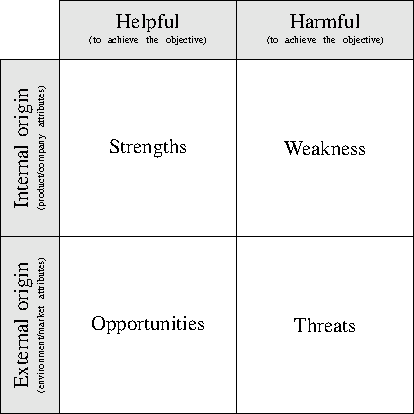
\includegraphics[scale=0.7]{SWOT}
\caption{An example of a SWOT analysis matrix}
\end{figure}
\column{0.5\textwidth}
To help an organisation with their \textbf{strategic planning}, a tool called SWOT analysis can be used.
\vspace{0.5cm}
 
\begin{block}{Definition: \textbf{S.W.O.T. Analysis}}
A systematic process which analyses the \textbf{strengths}, \textbf{weaknesses}, \textbf{opportunities}, and \textbf{threats} of an organisation.
\end{block}
\end{columns}
\end{frame}

%------------------------------------------------
\begin{frame}
\frametitle{SWOT Analysis}
The workings of a SWOT analysis can be best seen by way of example. Consider this website that you are on now. A group of people decided to make this course and host it on this web platform. They might determine the following based on a SWOT analysis:\\
\vspace{0.5cm}
\textbf{Strengths}
\begin{itemize}
\item As experienced teaching professionals, the group has many years experience building course content to direct students towards learning outcomes;
\item Many in the group have advanced interpersonal skills;
\item The group members are mostly comprised of engineering academics, which provides a high level of technical skill to develop the hosting platform;
\item Some members of the group possess strong management skills, and have previously directed successfully completed projects.
\end{itemize}
\end{frame}

%------------------------------------------------
\begin{frame}
\frametitle{SWOT Analysis}
\textbf{Weaknesses}
\begin{itemize}
\item There is little marketing experience in the group, and no clear marketing strategy;
\item There is little money to invest in new projects;
\item There is little legal expertise in the group.
\end{itemize}
\vspace{0.5cm}
\textbf{Opportunities}
\begin{itemize}
\item There are 11 million users on Open EdX websites, and another 11 million on the EdX site meaning that Charles Darwin University's School of Engineering may be able to reach a wider audience.
\item The online learning market is still not fully developed and there exists many opportunities for innovation.
\end{itemize}
\end{frame}
%------------------------------------------------
\begin{frame}
\frametitle{SWOT Analysis}
\textbf{Threats}
\begin{itemize}
\item Students may prefer traditional \textit{on campus} modes of learning.
\item There are many new companies creating businesses in this online learning space, which could lead to market saturation for this product.
\item The academic community may strongly oppose new modes of teaching and learning.
\end{itemize}
\vspace{0.25cm}
\textbf{Potential Projects}\\
The group, based on the SWOT analysis, might outline potential projects as follows:
\begin{itemize}
\item Find a legal expert to help them create the terms and conditions for users of the website;
\item Find a marketing expert who can help them run a successful marketing campaign for the newly developed website;
\item Contribute to research papers exploring the outcomes of online learning to raise the profile of the project in the academic community.
\end{itemize}
\end{frame}
%------------------------------------------------
\begin{frame}
\frametitle{SWOT Analysis}
\textbf{SWOT Analysis Using A Mind Map}\\
An alternative to the matrix method of performing a SWOT analysis is to use a mind map, as shown in the figure below.
\begin{figure}
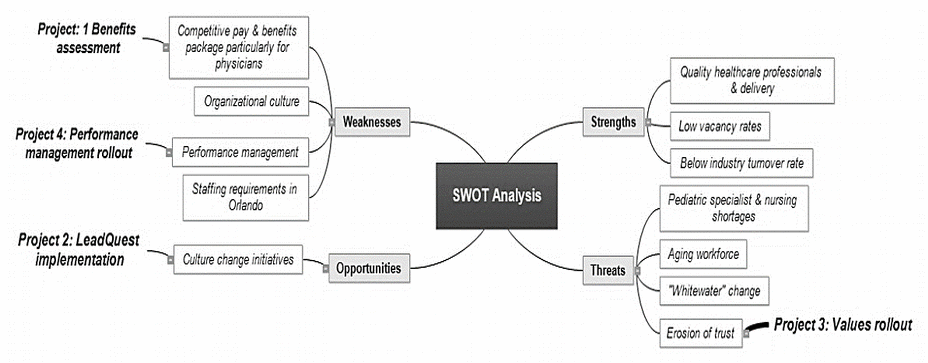
\includegraphics[scale=0.5]{swot_mind_map}
\caption{An example of a SWOT analysis performed using a mind map}
\end{figure}
\end{frame}
%------------------------------------------------

\begin{frame}[fragile]
\frametitle{Mind Mapping Software}
\begin{itemize}
\item There are a number of videos that instruct on how to create a mind map. Videos by Tony Buzan, author of \textit{The Mind Map Book: How to Use Radiant Thinking to Maximise Your Brain's untapped Potential}:\\
\begin{center}
\begin{verbatim}https://youtu.be/u5Y4pIsXTV0\end{verbatim}
\end{center}
\vspace{0.5cm}
\item Many free, online, applications allowing you to create beautiful mind maps are available on the internet. these will give you professional looking diagrams which you can include in your assignment. An example of one such site is:\\
\begin{center}
\begin{verbatim}https://bubbl.us/\end{verbatim}
\end{center}
\end{itemize}
\end{frame}

%------------------------------------------------
\begin{frame}
\frametitle{Four Stage Planning Process for Project Selection}
In addition to using a SWOT analysis some organisations often follow a detailed planning process for project selection. Typically a four-stage planning process is employed as shown in the diagram below:
\vspace{0.5cm}
\begin{figure}
\begin{enumerate}
\item Strategic Planning
\item Business Area Analysis
\item Project Planning
\item Resource Allocation
\end{enumerate}
\end{figure}
\end{frame}
%------------------------------------------------
\begin{frame}
\frametitle{Methods for Selecting Projects}
Recall that there are many potential projects, however, only a finite number of resources in an organisation to undertake these projects. Project selection is a vitally important process for successful businesses. Some of the tools for selecting projects are:
\vspace{0.5cm}
\begin{itemize}
\item Focus on competitive strategy and broad organisational needs;
\item Perform net present value analysis or other financial projections;
\item Use a weighted scoring model;
\item Implement a balanced scorecard;
\item Address problems, opportunities, and directives;
\item Consider project time frame;
\item Consider project priority.
\end{itemize}
\end{frame}
%------------------------------------------------
\begin{frame}
\frametitle{Methods for Selecting Projects}
\textbf{Focus on Competitive Strategy and Broad Organisational Needs}
\begin{columns}[t]
\column{0.40\textwidth}
\begin{block}{Definition: \textbf{Competitive Strategy}}
A \textbf{competitive strategy} is a strategy which a business will focus on to try and gain advantage over it's competitors.
\end{block}
\column{0.55\textwidth}
\begin{figure}
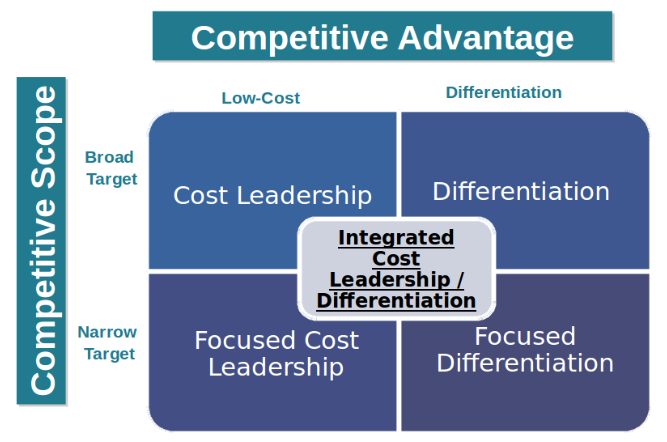
\includegraphics[scale=0.25]{comp_adv}
\caption{A matrix which shows some of the competitive strategies that organisations can adopt.}
\end{figure}
\end{columns}
\end{frame}
%------------------------------------------------
\begin{frame}
\frametitle{Methods for Selecting Projects}
\textbf{Focus on Competitive Strategy and Broad Organisational Needs}\\
\vspace{0.5cm}
There are a number of different \textbf{competitive strategies} in which an organisation could focus - some of the more common are:
\begin{itemize}
\item \textbf{Cost Leadership}: attract customers primarily because products or services are inexpensive. Examples include companies like Walmart or Aldi;
\item \textbf{Focus}: develop niche products and services for a particular market niche. An example includes the company Billabong focusing on surf culture.
\end{itemize}
\vspace{0.5cm}
If there is a consensus across the organisation that there is a \textbf{broad organisational need} for a project, then many times a company will make the funds available, and spend effort to ensure the successful completion of the project.
\end{frame}
%------------------------------------------------
\begin{frame}
\frametitle{Methods for Selecting Projects}
\textbf{Financial Projections: NPV Analysis}
\vspace{0.5cm}
\begin{block}{Definition: \textbf{Net Present Value Analysis}}
\textbf{Net present value (NPV) analysis} is a method of calculating the expected net monetary gain or loss from a project by discounting all expected future cash inflows and outflows to the present point in time.
\end{block}
\vspace{0.5cm}
\begin{itemize}
\item NPV means the return from a project exceeds the \textbf{opportunity cost of capital} - the return available by investing the capital elsewhere.
\item Projects with higher NPVs are preferred to projects with lower NPVs if all other factors are equal.
\end{itemize}
\end{frame}
%------------------------------------------------
\begin{frame}
\frametitle{Methods for Selecting Projects}
\textbf{Financial Projections: NPV Analysis - Calculating NPV}
\vspace{0.5cm}
\begin{itemize}
\item The calculations behind NPV come from the simple idea that time is money.
\item A dollar in your hand today is worth more than a dollar in your hand tomorrow.
\item This is because of the interest that the dollar in your hand today generates.
\item A project can be simplified to a series of cash flows occurring at different points in time - cash being received is positive cash flow, and cash going out of the project is negative cash flow.
\end{itemize}
\end{frame}
%------------------------------------------------
\begin{frame}
\frametitle{Methods for Selecting Projects}
\textbf{Financial Projections: NPV Analysis - Calculating NPV}\\
\vspace{0.5cm}
The main calculation for NPV analysis comes from the classical compounding interest formula shown below.
\vspace{0.2cm}
\begin{block}{Compound Interest Formula}
If $PV$ is the present value of some cash flow, $FV$ is the future value of some cash flow, $r$ is the compounding interest rate per period, and $n$ is the duration of the compounding, then:
\begin{align*}
FV = PV \cdot (1 + r)^n
\end{align*}
\end{block}
\vspace{0.2cm}
We can rearrange the formula shown above in order to discount cash flows to some previous time period:
\begin{align*}
PV = \frac{FV}{(1+r)^n}
\end{align*}
\end{frame}
%------------------------------------------------
\begin{frame}
\frametitle{Methods for Selecting Projects}
\textbf{Financial Projections: Steps for Calculating NPV}\\
\vspace{0.5cm}
\begin{enumerate}
\item Determine the estimated costs and benefits for the life of the project and the products it produces.
\item Subtract the costs from the benefits for each year to get a total cash flow for the given time period.
\item Determine the \textbf{discount rate}.
\item Discount each cash flow back to the start of the project and add them together - this figure is the NPV.
\end{enumerate}
\vspace{0.5cm}
\begin{block}{Definition: \textbf{Discount Rate}}
A \textbf{discount rate} is the rate used in discounting future cash flows.
\end{block}
\end{frame}
%------------------------------------------------
\begin{frame}
\frametitle{Methods for Selecting Projects}
\textbf{Financial Projections: NPV Considerations}\\
\vspace{0.5cm}
\begin{columns}
\column{0.45\textwidth}
\begin{itemize}
\item The discount rate can vary, based on the prime rate and other economic considerations;
\item Costs can be thought of as negative cash flows.
\item NPV is an attractive metric to use for project selection, however, it is often not the sole project selection method that is employed in industry.
\end{itemize}
\column{0.5\textwidth}
\begin{figure}
\frame{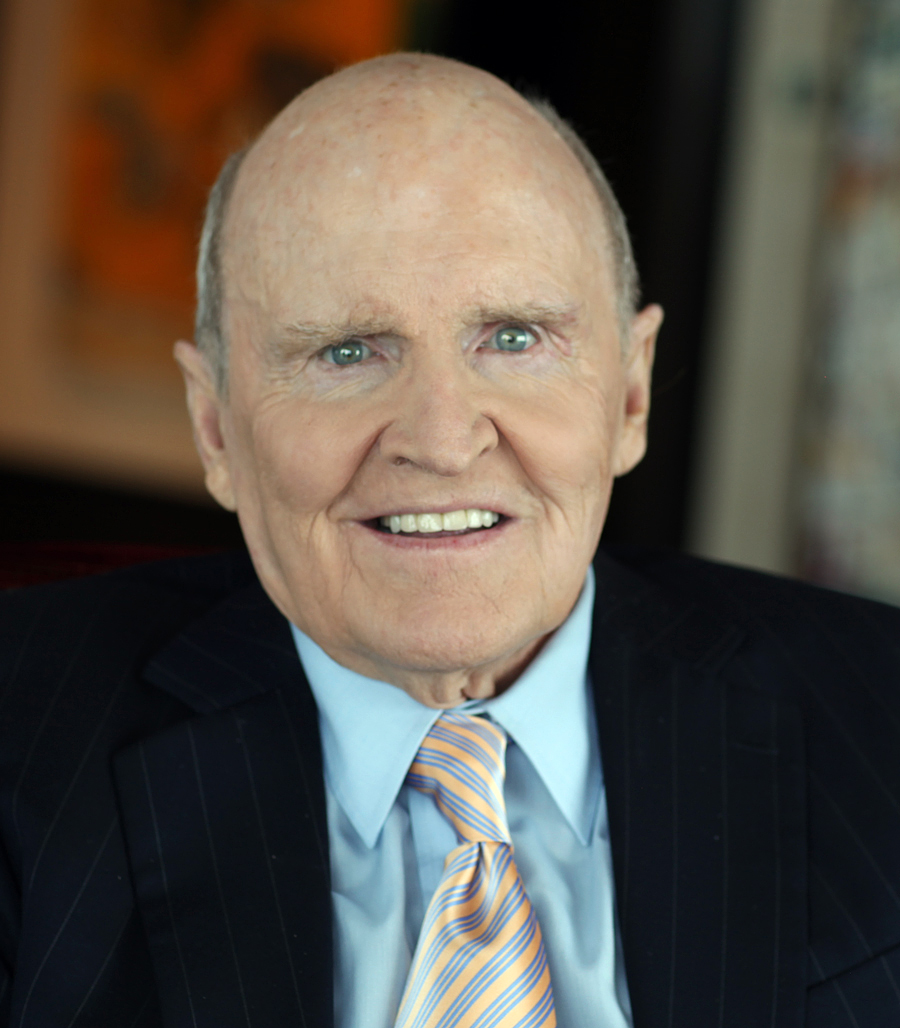
\includegraphics[scale=0.1]{JackWelchApril2012}}
\caption{Jack Welch, former CEO of G.E., is considered to be one of leaders in the rise of popularity surrounding shareholder value throughout the 1990s.}
\end{figure}
\end{columns}
\end{frame}
%------------------------------------------------
\begin{frame}
\frametitle{Methods for Selecting Projects}
\textbf{Financial Projections: Return on Investment (ROI)}\\
\vspace{0.5cm}
\begin{block}{Definition: \textbf{Return on Investment (ROI)}}
Return on investment is a simple calculation in which the total project costs are subtracted from the total project benefits, which is then divided by the total project costs.
\end{block}
\vspace{0.5cm}
\begin{example}[ROI Calculation]
Suppose that you spend \$100 on a project, and the total benefits that you receive back from this project are valued at \$110. The ROI would be as follows:
\begin{align*}
ROI = \frac{110 - 100}{100} = 0.10 = 10\%
\end{align*}
\end{example}
\end{frame}
%------------------------------------------------
\begin{frame}
\frametitle{Methods for Selecting Projects}
\textbf{Financial Projections: Return on Investment (ROI)}\\
\vspace{0.5cm}
\begin{itemize}
\item Note that ROI is always a percentage, and the higher the ROI, the better.
\item Many organisations have a \textbf{required rate of return} for projects - the minimum acceptable rate of return on an investment.
\item The \textbf{internal rate of return} can be found by determining the discount rate which results in an NPV of zero for the project.
\end{itemize}
\end{frame}
%------------------------------------------------
\begin{frame}
\frametitle{Methods for Selecting Projects}
\textbf{Financial Projections: Payback Period}\\
\vspace{0.5cm}
\begin{block}{Definition: \textbf{Payback Period}}
The \textbf{payback period} is the amount of time it will take to recoup, in the form of net cash inflows, the total dollars invested in the project.
\end{block}
\vspace{0.5cm}
\begin{itemize}
\item Payback period analysis determines how much time will lapse before accrued benefits overtake accrued and continuing costs.
\item Payback occurs in the year when the cumulative benefits minus the costs reach zero.
\item The shorter the payback period the better.
\end{itemize}
\end{frame}
%------------------------------------------------
\begin{frame}
\frametitle{Methods for Selecting Projects}
\textbf{Financial Projections: Payback Period}\\
\begin{figure}
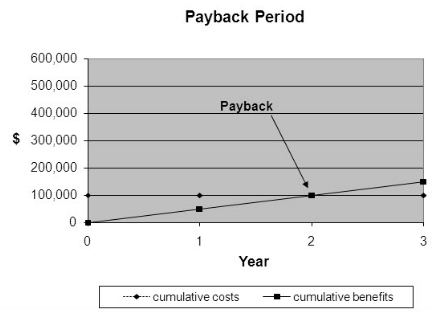
\includegraphics[scale=0.5]{payback}
\caption{Diagram showing both cumulative benefits and cumulative costs over time. The intersection of these two curves is the time period in which the project has paid back the overall investment.}
\end{figure}
\end{frame}
%------------------------------------------------
\begin{frame}
\frametitle{Methods for Selecting Projects}
\textbf{Weighted Scoring Models}\\
\vspace{0.5cm}
\begin{block}{Definition: Weighted Scoring Model}
A \textbf{weighted scoring model} is a tool that provides a systematic process for selecting projects based on many criteria.
\end{block}
\vspace{0.5cm}
To create a weighted scoring model:
\begin{enumerate}
\item Identify criteria important to the project selection process;
\item Assign a weight to each criterion (so they add up to 100 percent);
\item Assign numerical scores to each criterion for each project;
\item Calculate the weighted scores by multiplying the weight for each criterion by its score and adding the resulting values.
\end{enumerate}
\end{frame}
%------------------------------------------------
\begin{frame}
\frametitle{Methods for Selecting Projects}
\textbf{Weighted Scoring Models - Example}\\
\vspace{0.5cm}
\begin{figure}
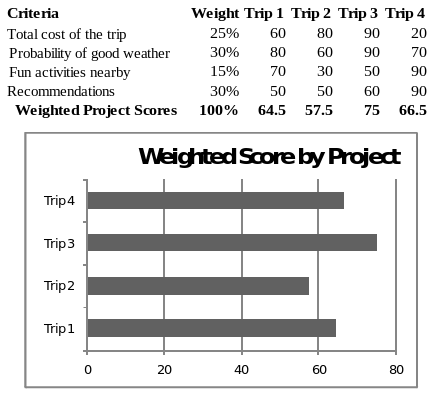
\includegraphics[scale=0.4]{weighted_scoring}
\caption{ur mum}
\end{figure}
\end{frame}
%------------------------------------------------
\begin{frame}
\frametitle{Methods for Selecting Projects}
\textbf{Implementing a Balanced Scorecard}\\
\vspace{0.5cm}
\begin{block}{Definition: \textbf{Balanced Scorecard}}
A \textbf{balanced scorecard} is a methodology that converts an organisation's value drivers - such as customer service, innovation, operational efficiency, and financial performance - to a series of defined metrics.
\end{block}
\vspace{0.5cm}
This method of project selection was developed by Dr. Robert Kaplan and Dr. David Norton to help select and manage projects that align with business strategy. For more information on this visit:
\begin{center}
\url{www.balancedscorecard.org}
\end{center}
\end{frame}
%------------------------------------------------
\begin{frame}
\frametitle{Methods for Selecting Projects}
\textbf{Implementing a Balanced Scorecard - Example}\\
\vspace{0.1cm}
\begin{center}
\scalebox{0.8}{
\begin{tcolorbox}
\textbf{Nemours Children's Hospital Case Study}\\
\begin{itemize}
\item \textbf{Mission}: to provide leadership, institutions, and services to restore and improve the health of children through care and programs not readily available, with one high standard of quality and distinction regardless of the recipient's financial status.
\item \textbf{Vision}: freedom from disabling conditions
\item \textbf{Goals}:
\begin{itemize}
	\item Be a leader in improving children's health through our integrated health system; becoming a pre-eminent voice for children
	\item Care for each and every child as if they were our own
	\item Be a great place to work
	\item Be effective stewards of all of our assets, continually improving them to advance our mission.
\end{itemize}
\end{itemize}
\end{tcolorbox}
}
\end{center}
\end{frame}
%------------------------------------------------
\begin{frame}
\frametitle{Methods for Selecting Projects}
\textbf{Implementing a Balanced Scorecard - Example}\\
\vspace{0.5cm}
\begin{figure}
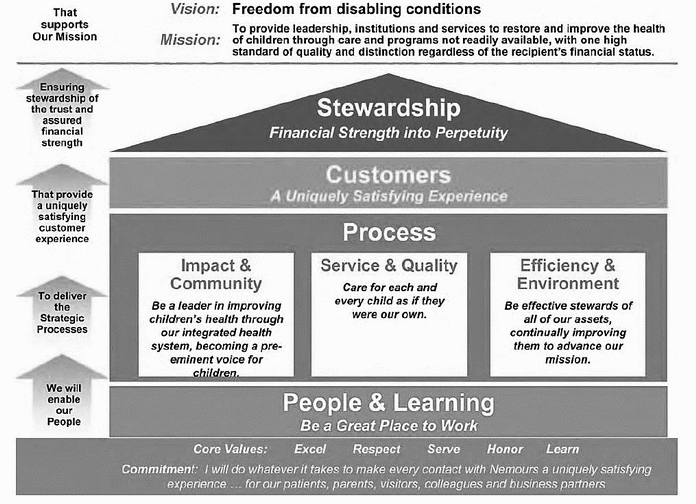
\includegraphics[scale=0.4]{balanced_score}
\caption{An example of a balanced scorecard for Nemours.}
\end{figure}
\end{frame}
%------------------------------------------------
\begin{frame}
\frametitle{Methods for Selecting Projects}
\textbf{Problems, Opportunities, and Directives}\\
\vspace{0.5cm}
Another method for selection of projects is based on the project's response to a \textbf{problem}, an \textbf{opportunity}, or a \textbf{directive}.
\vspace{0.2cm}
\begin{block}{Definition: \textbf{Problem}}
A \textbf{problem} is an undesirable situation that can prevent an organisation from achieving its goals - can be current or anticipated.
\end{block}
\vspace{0.2cm}
\begin{block}{Definition: \textbf{Opportunity}}
An \textbf{opportunity} is a chance to improve the organisation.
\end{block}
\vspace{0.2cm}
\begin{block}{Definition: \textbf{Directive}}
A \textbf{directive} is a new requirement imposed by management, government, or some external influence.
\end{block}
\end{frame}

%------------------------------------------------
\begin{frame}
\frametitle{Methods for Selecting Projects}
\textbf{Project Time Frame}
\vspace{0.1cm}
\begin{itemize}
\item Another approach to project selection is based on the time it will take to complete a project or the date by which it must be done.
\item Some potential projects must be finished within a specific time period - if they cannot be finished by this set date, they are no longer valid projects.
\item Some projects can be completed very quickly - within a few weeks, days, or even minutes. However, even though many projects can be completed quickly, it is still important to prioritise them.
\end{itemize}
\vspace{0.5cm}
\textbf{Project Priority}
\vspace{0.1cm}
\begin{itemize}
\item Many organisations prioritize projects as being high, medium, or low priority based on the current business environment.
\item Organisations should always focus on high-priority projects.
\end{itemize}
\end{frame}

%------------------------------------------------
\begin{frame}
\frametitle{Project Program Selection}
Recall from a previous lecture that a \textbf{program} is defined as a group of projects managed in a coordinated way to obtain benefits and control not available from managing them individually.
\vspace{0.3cm}
\begin{figure}
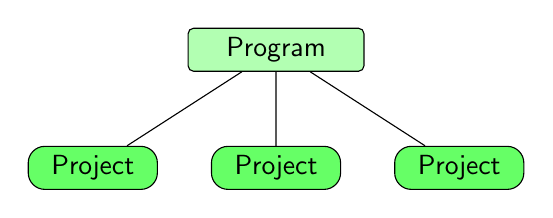
\begin{tikzpicture}
	\tikzset{
	  basic/.style  = {draw, text width=2cm, font=\sffamily, rectangle},
	  root/.style   = {basic, rounded corners=2pt, thin, align=center,
	                   fill=green!30},
	  level 2/.style = {basic, rounded corners=6pt, thin,align=center, fill=green!60,
	                   text width=4em},
	  level 3/.style = {basic, thin, align=left, fill=pink!60, text width=6.5em}
	}
	
	level 1/.style={sibling distance=40mm},
	  edge from parent/.style={->,draw},
	  >=latex]
	  
	\node[root] {Program}
	% The first level, as children of the initial tree
	  child {node[level 2, left] (c1) {Project}}
	  child {node[level 2] (c2) {Project}}
	  child {node[level 2, right] (c3) {Project}};
\end{tikzpicture}
\caption{The basic structure of a program}
\end{figure}
An organisation using a program management structure, when categorising each project, needs to determine if the project can be allocated to an existing program or if a new program needs to be created.

\end{frame}

%------------------------------------------------
\begin{frame}
\frametitle{Project Portfolio Selection}
Recall from a previous lecture that \textbf{project portfolio management} is defined as an emerging business strategy in which organisations group and manage projects and programs as a portfolio of investments that contribute to the entire enterprise's success.
\begin{figure}
\tikzset{
	  basic/.style  = {draw, text width=2cm, font=\sffamily, rectangle},
	  root/.style   = {basic, rounded corners=2pt, thin, align=center,
	                   fill=green!30},
	  level 2/.style = {sibling distance=40mm, basic, rounded corners=6pt, thin,align=center, fill=green!60,
	                   text width=4em},
	  level 3/.style = {sibling distance=40mm, basic, thin, align=left, fill=pink!60, text width=6.5em}
	}
\begin{tikzpicture}[
	level 1/.style={sibling distance=20mm},
	  edge from parent/.style={->,draw},
	  >=latex]
	  
	\node[root] {Portfolio}
	% The first level, as children of the initial tree
	  child {node[level 2, left] (c1) {Project}}
	  child {node[level 2] (c2) {Program}}
	  child {node[level 2] (c3) {Project}}
	  child {node[level 2, right] (c4) {Program}};
\end{tikzpicture}
\end{figure}
\begin{itemize}
\item It's crucial to focus on enterprise success when creating project portfolios;
\item There may be a need to cancel or put several projects on hold, reassign resources from one project to another, suggest changes in project leadership, or take other actions that might negatively affect individual projects or programs to help the organisation as a whole.
\end{itemize}
\end{frame}
%------------------------------------------------
\begin{frame}
\begin{center}
\huge The End
\end{center}
\end{frame}
\end{document} 